\renewcommand{\theequation}{\theenumi}
\begin{enumerate}
\numberwithin{equation}{enumi}

\item \begin{flushleft}
 $\vec{A}$ denotes the velocity of the boat and $
\vec{B}$ denotes the water current and $\vec{C}$ represents the resultant velocity. 
\end{flushleft}

\item \begin{align}
\vec{A} &=\myvec{0\\25} \label{eq:constr_a_motion_in_a_plane}\\
\vec{B} &=\myvec{8.6\\-5} \label{eq:constr_b_motion_in_a_plane}\\
\vec{C} &= \vec{A} + \vec{B}\\
\vec{C} &= \myvec{8.6\\20}
\end{align}

\item Magnitude of resulant velocity:
\begin{align}
\norm{\vec{C}} &= 21.8
\end{align}

\item Direction of resultant velocity:
\begin{align}
\cos{\theta} &= \frac{\brak{\vec{A}}^T\brak{\vec{C}}}{\norm{\vec{A}}\ \norm{\vec{C}}}\\
\theta &= 23.41\degree
\end{align}

\item \begin{flushleft}
$\therefore$ The resulant velocity is $21.8$ km/h at an angle of $23.41\degree$ east of north.
\end{flushleft}

\item \begin{figure}[!ht]
\centering
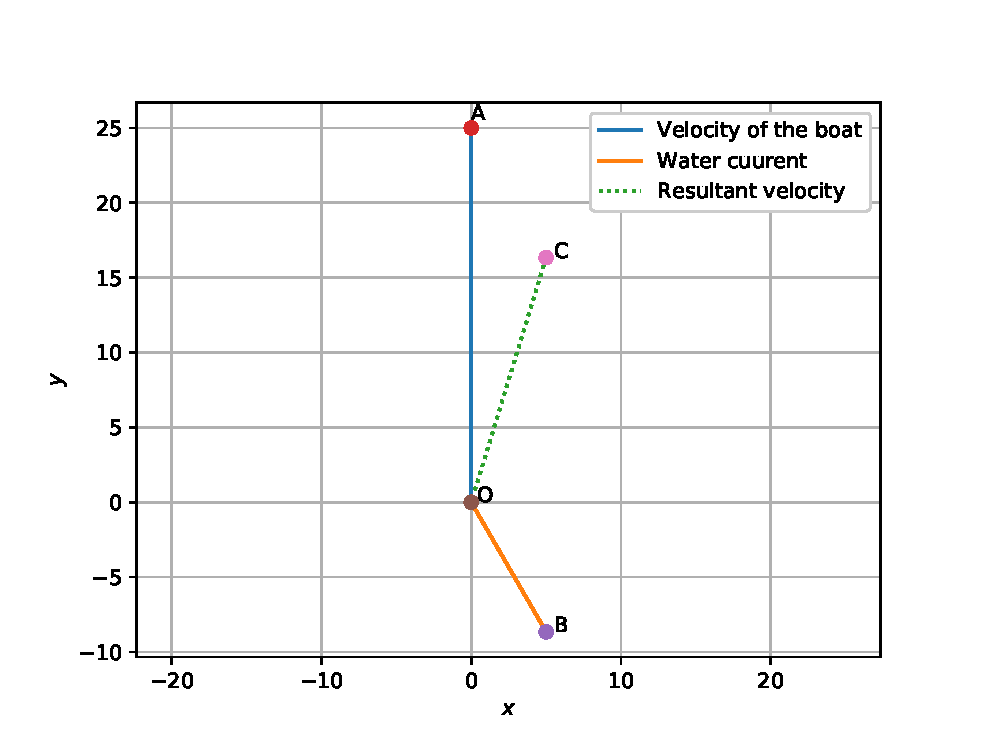
\includegraphics[width=\columnwidth]{./figs/line_ex/motion_in_a_plane/motion_plane.eps}
\caption{Vectorial representation of velocities generated using python}
\label{fig:motion_plane_motion_in_a_plane}
\end{figure} 

The following Python code generates Fig. \ref{fig:motion_plane_motion_in_a_plane}

\begin{lstlisting}
codes/line_ex/motion_in_a_plane/motion_plane.py
\end{lstlisting}

\end{enumerate}
